%
% Sección introducción a la criptografía, capítulo de antecedentes.
% Proyecto Lovelace.
%

\section{Introducción a la criptografía}

La palabra criptografía proviene de las etimologías griegas \textit{Kriptos}
(ocultar) y \textit{Graphos} (escritura), y es definida por la Real Academia
Española como el arte de escribir con clave secreta o de un modo enigmático.
De manera más formal se puede definir a la criptografía como la ciencia
encargada de estudiar y diseñar por medio de técnicas matemáticas, métodos y
modelos capaces de resolver problemas en la seguridad de la información, como
la confidencialidad de esta, su integridad y la autenticación de su origen.

  \subsection{Objetivos de la criptografía}

    La criptografía tiene como finalidad cumplir los siguientes cuatro
    servicios.

    \begin{enumerate}

      \item \textbf{Confidencialidad}

        Es el servicio encargado de mantener legible la información solo a
        aquellos que estén autorizados a visualizarla.

      \item \textbf{Integridad}

        Este servicio se encarga de evitar la alteración de la información de
        forma no autorizada, esto incluye la inserción, sustitución y
        eliminación de los datos.

      \item \textbf{Autenticación}

        Este servicio se refiere a la identificación tanto de las personas que
        establecen una comunicación, garantizando que cada una es quien dice
        ser; como del origen de la información que se maneja, garantizando la
        veracidad de la hora y fecha de origen, el contenido, tiempos de
        envío, entre otros.

      \item \textbf{No repudio}

        Es el servicio que evita que el autor de la información o de alguna
        acción determinada, pueda negar su validez, ayudando así a prevenir
        situaciones de disputa.

    \end{enumerate}

  \subsection{Criptoanálisis y ataques}

    La criptografía forma parte de una ciencia más general llamada
    criptología, la cual tiene otras ramas de estudio, como es el
    criptoanálisis que es la ciencia encargada de estudiar los posibles
    ataques a sistemas criptográficos, que son capaces de contrariar sus
    servicios ofrecidos.
    Los ataques que se realizan a sistemas criptográficos dependen de la 
    cantidad de recursos o conocimientos con los que cuenta el adversario 
    que realiza dicho ataque, dando así a la siguiente clasificación.

    \begin{enumerate}

      \item \textbf{Ciphertext-only attack}

        En este ataque el adversario sólo es capaz de obtener la información
        cifrada, y tratara de conocer su contenido en claro a partir de ella.
        Esta forma de atacar es la más básica, y todos los métodos
        criptográficos deben poder soportarla.

      \item \textbf{Known-plaintext attack}

        Esta clase de ataques ocurren cuando el adversario puede obtener pares
        de información cifrada y su correspondiente información en claro, y
        por medio de su estudio, trata de descifrar otra información cifrada
        para la cual no conoce su contenido.

      \item \textbf{Chosen-plaintext attack}

        Este ataque es muy parecido al anterior, con la diferencia de que en
        este el adversario es capaz de obtener los pares de información
        cifrada y en claro con el contenido que desee.

      \item \textbf{Adaptively-chosen-plaintext attack}

        En este ataque el adversario es capaz de obtener los pares de
        información cifrada y en claro con el contenido que desee y además 
        tiene amplio acceso o puede usar de forma repetitiva el mecanismo de
        cifrado.

      \item \textbf{Chosen and adaptively-chosen-ciphertext attack}
        En este caso el adversario puede elegir información cifrada y conocer
        su contenido, dado que tiene acceso a los mecanismos de descifrado.

    \end{enumerate}

  \subsection{Clasificación de la criptografía}

    La criptografía puede clasificarse de forma histórica en dos categorías,
    la criptografía clásica y la criptografía moderna. La criptografía clásica
    es aquella que se utilizó desde la antigüedad, teniéndose registro de su
    usado desde hace más 4000 años por los egipcios, hasta la mitad del siglo
    XX. En esta los métodos utilizados para cifrar eran variados, pero en su
    mayoría usaban la transposición y la sustitución, además de que la mayoría
    se mantenían en secretos. Mientras que la criptografía moderna es la que
    se inició después la publicación de la \textit{Teoría de la información}
    por Claude Elwood Shannon, dado que esta sentó las bases matemáticas para
    la criptología en general.

    Una manera de clasificar es de acuerdo a las técnicas y métodos empleados
    para cifrar la información, esta clasificación se puede observar en la
    siguiente figura.

    \begin{figure}[H]
      \begin{center}
        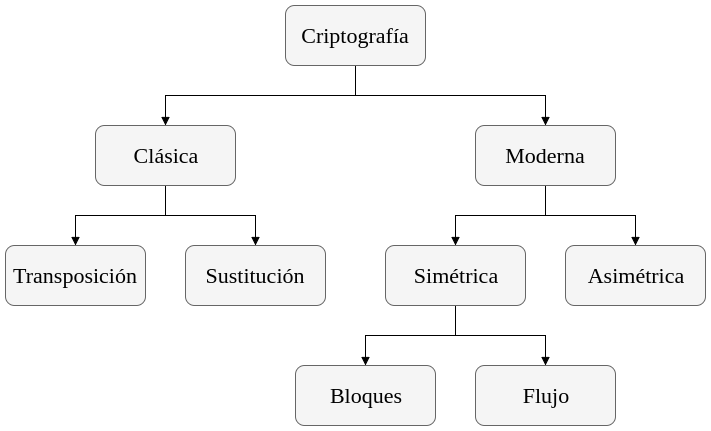
\includegraphics[width=0.7\linewidth]
          {contenidos/antecedentes/intro_img/clasificacion_cripto.png}
        \caption{Clasificación de la criptografía.}
      \end{center}
    \end{figure}

    Adentrándose en la clasificación de la criptografía clásica, se tienen los 
    cifrados por transposición, los cuales se basan en técnicas de permutación 
    de forma que los caracteres de la información en claro se reordenen 
    mediante algoritmos específicos, y los cifrados por sustitución, que 
    utilizan técnicas de modificación de los caracteres por otros
    correspondiente a un alfabeto específico para el cifrado.

    En cuanto a la criptografía moderna, esta tiene dos vertientes, la
    criptografía simétrica o de llave secreta y la asimétrica o de llave
    pública. Hablando de la primer vertiente, se puede decir que es aquella
    que utiliza un modelo matemático para cifrar y descifrar un mensaje
    utilizando únicamente una llave que permanece secreta.

    \begin{figure}[H]
      \begin{center}
        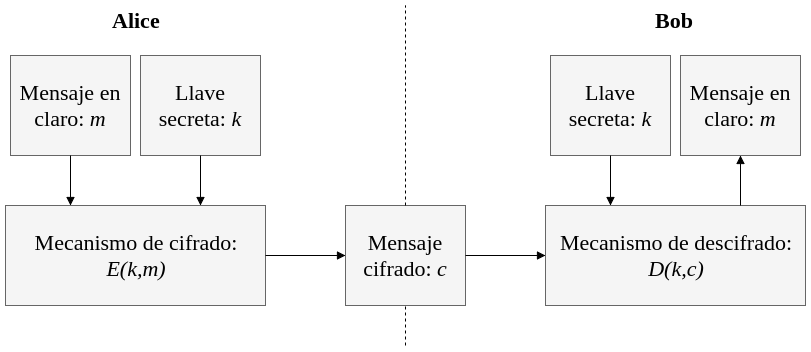
\includegraphics[width=0.8\linewidth]
          {contenidos/antecedentes/intro_img/cripto_simetrica.png}
        \caption{Canal de comunicación con criptografía simétrica.}
      \end{center}
    \end{figure}

    En la figura anterior se puede observar el proceso para establecer una
    comunicación segura por medio de la criptografía simétrica. Primero, tanto
    Alice como Bob deben de establecer una llave única y compartida $k$, para
    que después, Alice, actuando como el emisor, cifre un mensaje $m$ usando
    la llave $k$ por medio del algoritmo de cifrado $E(k,m)$ para obtener el
    mensaje cifrado $c$ y enviárselo a Bob. Posteriormente Bob, como receptor,
    se encarga de descifrar $c$ con ayuda de la llave $k$ por medio del
    algoritmo de descifrado $D(k,c)$ para obtener el mensaje original $m$.

    Entre los beneficios de este tipo de criptografía está su utilidad para
    cifrar archivos personales, su relativa facilidad de uso y para garantizar
    la confidencialidad e integridad debido al uso de una llave, y su rapidez, 
    pero en contraparte, su uso genera problemas para organizar y compartir 
    las llaves secretas de una forma segura y eficiente.

    Ahora, adentrándose en la criptografía asimétrica, se tiene que su idea
    principal es el uso de 2 llaves distintas para cada persona, una llave
    pública para cifrar que esté disponible para cualquier otra persona, y una
    llave privada para descifrar, que se mantiene disponible solo para su
    propietario.

    El proceso para establecer una comunicación segura por medio de este tipo
    de criptografía es el siguiente: primero, Alice nuevamente como el emisor,
    cifra un mensaje $m$ con la llave pública de Bob $pk$ usa el algoritmo de 
    cifrado $E(pk,m)$ para obtener $c$ y enviarlo. Después Bob como receptor, 
    se encarga de descifrar $c$ por medio del algoritmo de descifrado 
    $D(sk,c)$ haciendo uso de su llave privada $sk$. Este proceso se refleja 
    gráficamente el la siguiente figura.

    \begin{figure}[H]
      \begin{center}
        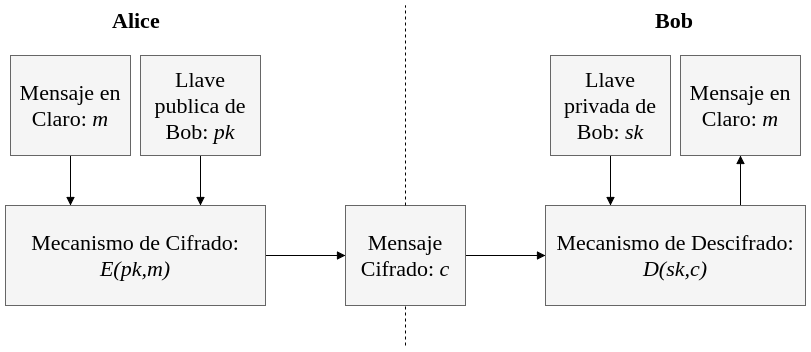
\includegraphics[width=0.8\linewidth]
          {contenidos/antecedentes/intro_img/cripto_asimetrica.png}
        \caption{Canal de comunicación con criptografía asimétrica.}
      \end{center}
    \end{figure}

    Entre los uso que se le da a esta criptografía está el mantener la
    distribución de llaves privada segura, y establecer métodos que garantizan
    la autenticación y el no repudio, como por ejemplo en las firmas y
    certificados digitales.
